\chapter{Augmenting Nanomolar High-Throughput Screening with Machine Learning for Lead Optimisation}\label{ch:testing}

Typically, testing a drug candidate involves obtaining a pure sample of the molecule, and then mixing it in solution with the protein target under study to measure its bioactivity via an assay. While necessary for maximum accuracy, compound purification can be time-consuming and costly, particularly for chiral molecules. In collaboration with the London Lab at The Weizmann Institute of Science, we investigated whether we needed compound purification at all for training machine learning bioactivity models by using non-purified compound assays. Focusing on a particular scaffold synthesised with an amide coupling as the final step, we added the acid and amine reactants directly in solution with the protein to obtain an assay reading from the crude reaction mixture. By skipping the purification step, this allowed us to quickly screen a library of < 300 > amines with the same acid in high-throughput which we used to train RF and GP models. Leave-one-out validation on the training data correctly identified false negatives, and a prospective virtual screen of EnamineREAL with the trained models returned top hits with similar potency and better pharmacokinetic properties.

Machine learning (ML) has seen great advances over the past two decades in drug discovery and development, from protein-ligand interactions to novel scaffold generation to virtual screening of pharmacokinetic properties and toxicity.1-5 Generally, ML algorithms are tasked with prediction of specific target(s) with the endeavor that the faster predictions in silico will lead to faster pharmaceutical development. Hastening drug development is a key factor in reducing the overall cost of pharmaceutics, where it can reach up to \$2 billion to bring a compound to market.1 However, one overlooked area in this development cycle is ML applied as a filtering protocol for initial lead discovery, despite reports that ML methods often implicitly identify false positives and false negatives.6,7 Crude activity screening (assuming some level of introduction by Mihajlo is given previously) is a logical area to apply such techniques as noise and false hits/misses play a substantial role in obscuring valuable data. We hypothesized that combining two robust ML methodologies, Gaussian Processes (GPs) and Random Forests (RFs), could be used to identify hidden gems (false negatives) and overlooked molecules (low activity positives). Both GPs and RFs have been utilized in numerous chemoinformatics tasks, with several precedents in pharmaceutics development, making both ideal for predicting activity of novel compounds.8-12 Given the difference in approach to modeling for GPs and RFs, it was hypothesized that a combination of the two would lead to a highly robust framework; a compound predicted to have low activity from both a GP and a RF is likely to be inactive and likewise a compound with high predicted activity from both the GP and RF is likely potent.

\begin{figure}
    \centering
             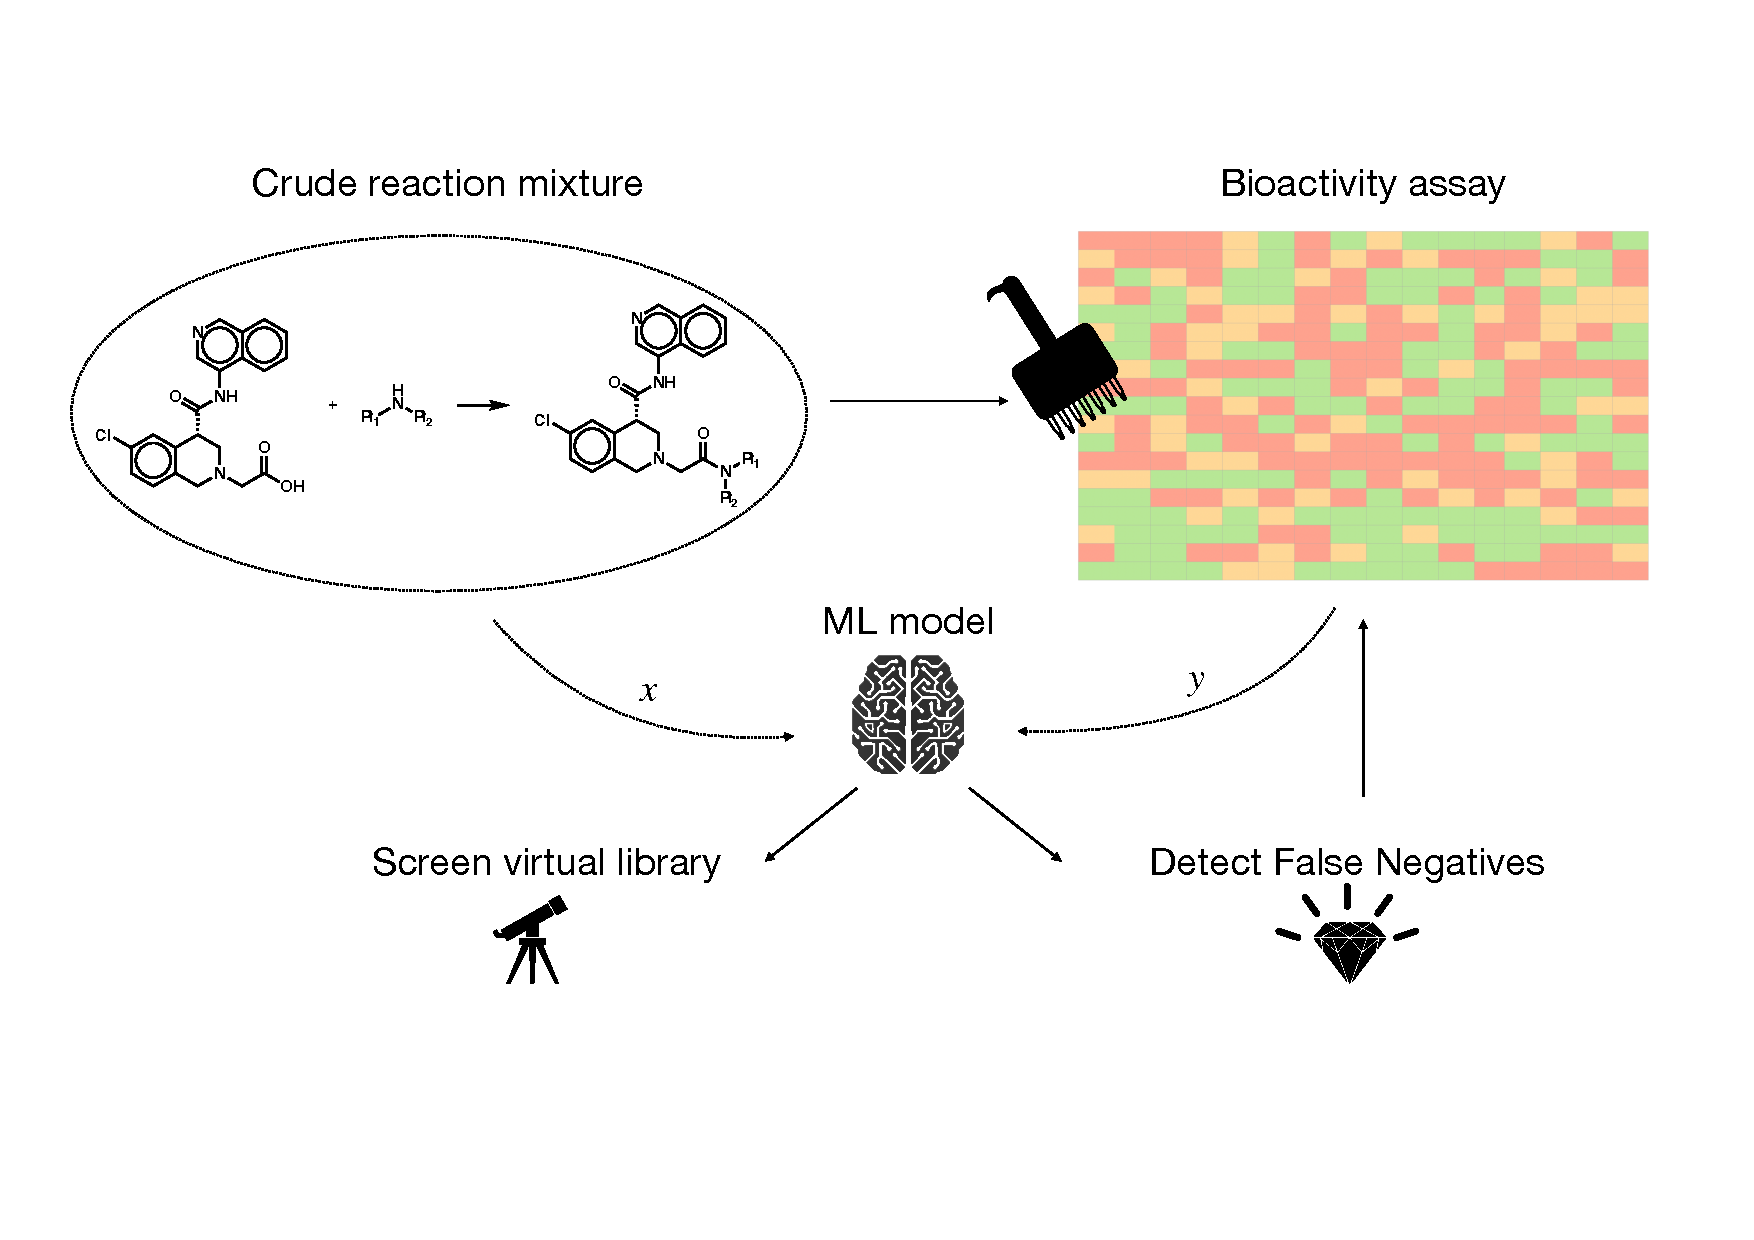
\includegraphics[width=\textwidth]{Chapters/Crude/Figs/schematic.pdf}
        \caption{Schmeatic of workflow.}
        \label{fig:leave-one-out}
    \end{figure}

Thus, we separately trained a GP and RF on the crude inhibition data, identifying 5 compounds which had predicted activity from both the GP and RF but no crude activity. We suspected that these were false negatives and re-synthesized, purified, and re-tested them with full dose-response curves to obtain IC50 inhibition values. This revealed that one of them was active with IC50 = 0.113\uM (ASAP-0000204). (needs a nice sentence to round it off).

\begin{figure}
    \centering
             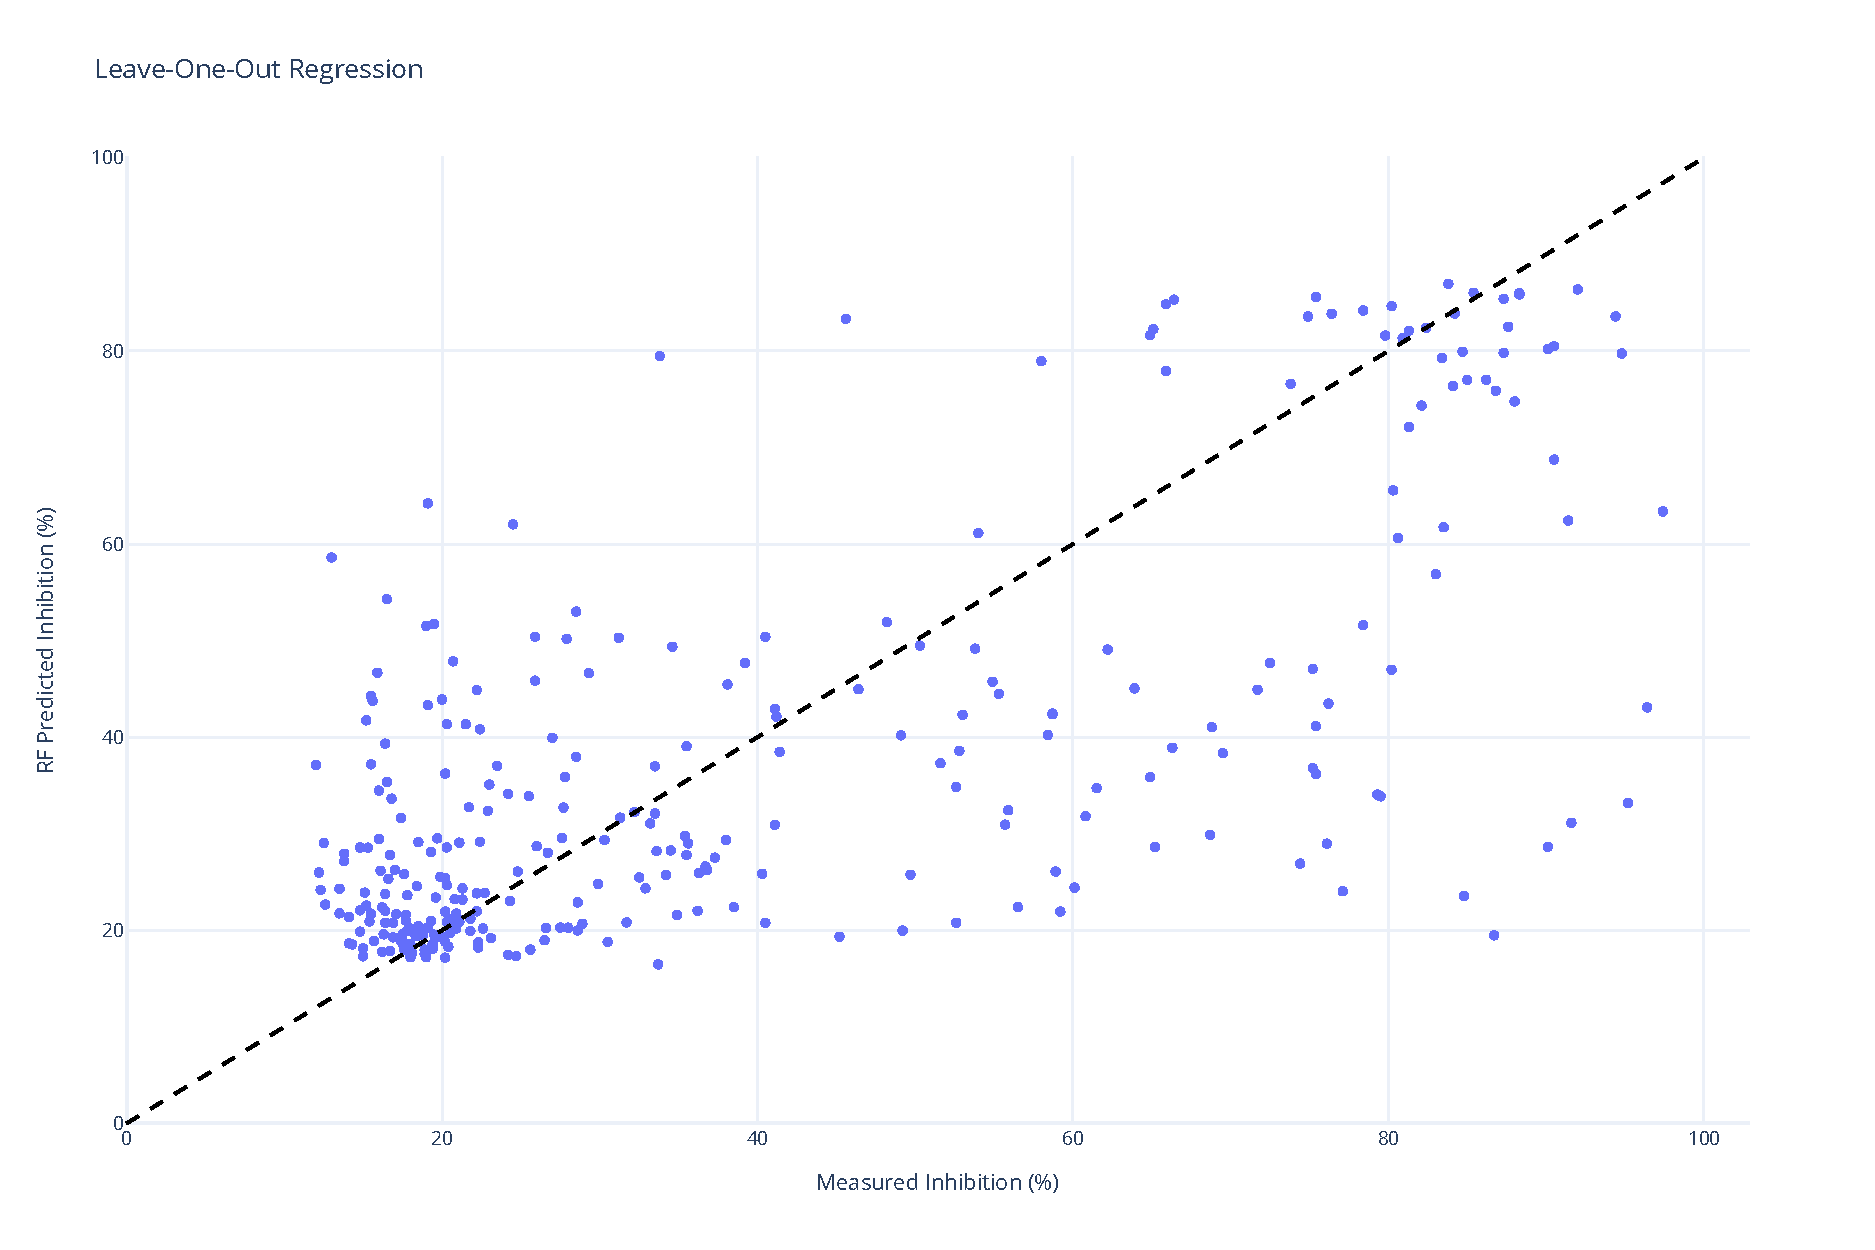
\includegraphics[width=\textwidth]{Chapters/Crude/Figs/rf.pdf}
        \caption{Leave one out regression. }
        \label{fig:leave-one-out}
    \end{figure}
    
Looking forward, we test the ability of the trained models to extrapolate to novel compounds by prospectively screening an external library of amides. We virtually enumerate primary and secondary amine building blocks from Enamine with the same carboxylic acid substructure from the crude activity screening. This results in a library of ~62,800 amides which were scored by the trained GP and RF models, and we select the top 20 compounds with high predicted activity for both the GP and RF for synthesis and assaying to obtain IC50 values. Gratifyingly, the top 2 ML compounds showed promising average IC50 values of 0.0525\uM (ASAP-0000169) and 0.075\uM (ASAP-0000211), respectively. The top 2 most potent molecules based off of the crude inhibition values were compounds that, whilst active at IC50 = 0.034\uM (ASAP-0000221) and IC50 = 0.064\uM (ASAP-0000164), contained the toxic benzene-1,4-diamine motif that is generally avoided.13 The top 2 compounds without the aforementioned motif derived from only crude inhibition values had similar pure compound IC50 values to our framework's identified compounds, 0.046\uM (ASAP-0000155) and 0.064\uM (ASAP-0000225), respectively. This result highlights ML's ability to identify promising yet overlooked scaffolds without compromising potency. 

\begin{figure}
    \centering
             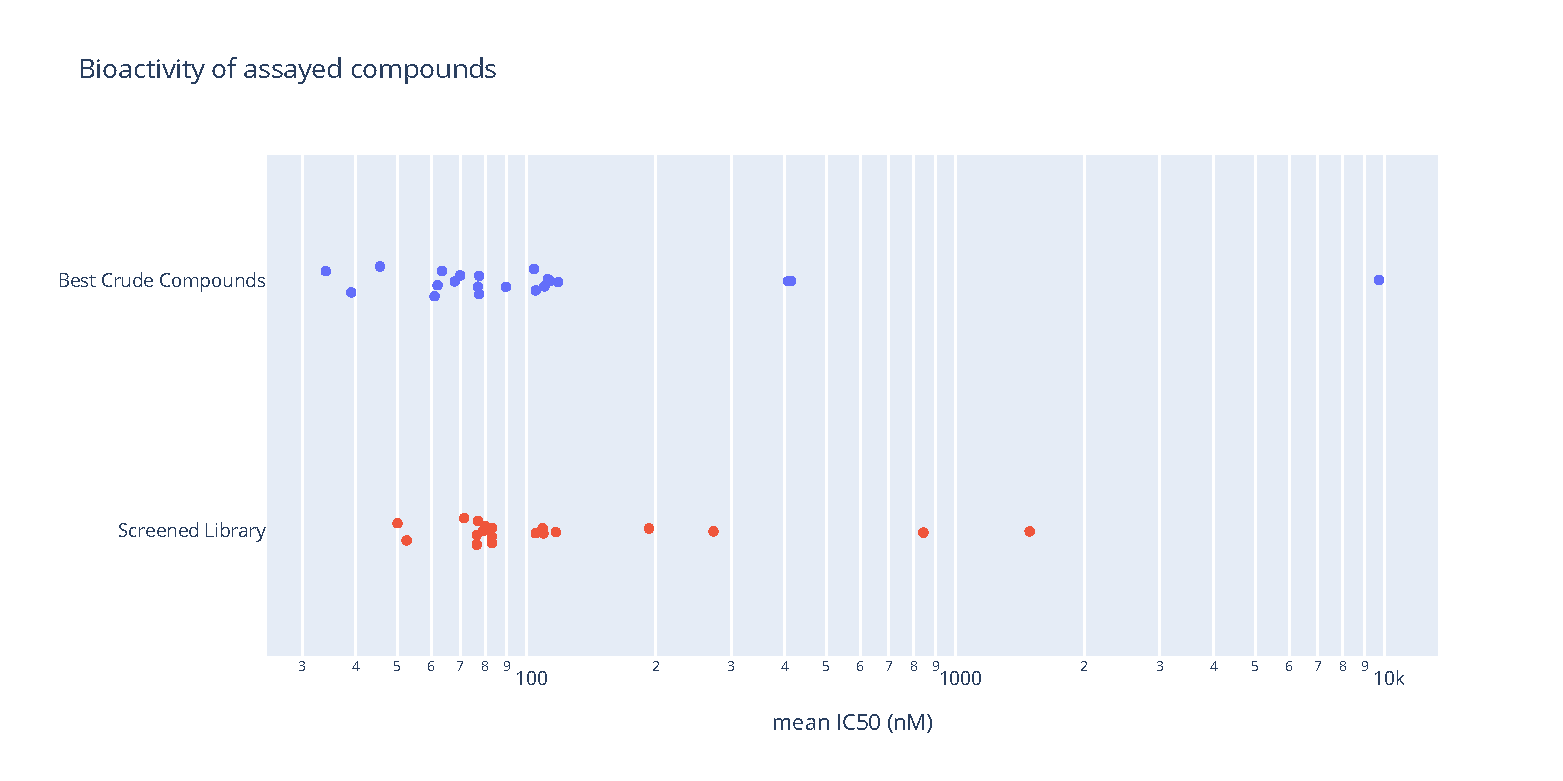
\includegraphics[width=\textwidth]{Chapters/Crude/Figs/strip_plot.pdf}
        \caption{Plot of mean IC50 values.}
        \label{fig:strip}
    \end{figure}

Figure 4 - top 2 crude, false negative?

References:

1	Selvaraj, C., Chandra, I. \& Singh, S. K. Artificial intelligence and machine learning approaches for drug design: challenges and opportunities for the pharmaceutical industries. Molecular Diversity 26, 1893-1913, doi:10.1007/s11030-021-10326-z (2022).
2	Göller, A. H. et al. Bayer’s in silico ADMET platform: A journey of machine learning over the past two decades. Drug discovery today 25, 1702-1709 (2020).
3	Lavecchia, A. Machine-learning approaches in drug discovery: methods and applications. Drug Discovery Today 20, 318-331, doi:https://doi.org/10.1016/j.drudis.2014.10.012 (2015).
4	Lipinski, C. F., Maltarollo, V. G., Oliveira, P. R., Da Silva, A. B. \& Honorio, K. M. Advances and perspectives in applying deep learning for drug design and discovery. Frontiers in Robotics and AI 6, 108 (2019).
5	Vamathevan, J. et al. Applications of machine learning in drug discovery and development. Nature Reviews Drug Discovery 18, 463-477, doi:10.1038/s41573-019-0024-5 (2019).
6	Ardila, D. et al. End-to-end lung cancer screening with three-dimensional deep learning on low-dose chest computed tomography. Nature medicine 25, 954-961 (2019).
7	Ryu, J. Y., Lee, M. Y., Lee, J. H., Lee, B. H. \& Oh, K.-S. DeepHIT: a deep learning framework for prediction of hERG-induced cardiotoxicity. Bioinformatics 36, 3049-3055 (2020).
8	Jiménez-Luna, J., Grisoni, F. \& Schneider, G. Drug discovery with explainable artificial intelligence. Nature Machine Intelligence 2, 573-584, doi:10.1038/s42256-020-00236-4 (2020).
9	Reker, D. \& Schneider, G. Active-learning strategies in computer-assisted drug discovery. Drug discovery today 20, 458-465 (2015).
10	Kapsiani, S. \& Howlin, B. J. Random forest classification for predicting lifespan-extending chemical compounds. Scientific Reports 11, 13812, doi:10.1038/s41598-021-93070-6 (2021).
11	Svetnik, V. et al. Random Forest: A Classification and Regression Tool for Compound Classification and QSAR Modeling. Journal of Chemical Information and Computer Sciences 43, 1947-1958, doi:10.1021/ci034160g (2003).
12	Kang, B., Seok, C. \& Lee, J. Prediction of Molecular Electronic Transitions Using Random Forests. Journal of Chemical Information and Modeling 60, 5984-5994, doi:10.1021/acs.jcim.0c00698 (2020).
13	Kumar, M. S., Tamilarasan, R. \& Sreekanth, A. 4-Salicylideneamino-3-methyl-1,2,4-triazole-5-thione as a sensor for aniline recognition. Spectrochimica Acta Part A: Molecular and Biomolecular Spectroscopy 79, 370-375, doi:https://doi.org/10.1016/j.saa.2011.03.030 (2011).

